\ifdefined\PROCINCLUDED
%
\else
%%% Please, do not change any of the following parameters.
\documentclass[b5paper,twoside,11pt]{article}
\usepackage[utf8]{inputenc}
\usepackage{geometry}
\voffset=-0.04cm
\headheight=0.6cm
\headsep=0.65cm
\textheight=19.5cm
\footskip=1.25cm
\voffset=-0.04cm
\textwidth=12.6cm
\marginparsep=0cm
\oddsidemargin=0cm
\evensidemargin=0cm
\marginparwidth=0cm
\usepackage{fancyhdr}
\usepackage{url}
\usepackage{graphicx}
\usepackage{mathptmx}
\usepackage{amsmath}
\usepackage{float}
\usepackage{subcaption}
\usepackage{placeins}
\usepackage{gensymb}
\usepackage{enumitem}
\usepackage{blindtext} 
\usepackage{tocloft}
\usepackage[labelsep=period]{caption}
\usepackage{caption}
\usepackage{subcaption}
\captionsetup[table]{skip=7pt}
\captionsetup[figure]{skip=6pt}
\fancyhead{}
\fancyfoot{}
\fancyfoot[LE]{\thepage}
\fancyfoot[RO]{\thepage}
\renewcommand{\headrulewidth}{0.4pt}
\renewcommand{\footrulewidth}{0pt}
\date{}
\def \papertitle#1{\title{#1}}
\pagestyle{fancy}
\def\insertauthor#1#2{
	\begin{minipage}[t]{.45\textwidth}
		\centering
		{\em#1} \\ \vspace*{0.25em}
		#2 \\ \vspace*{1.25em}
	\end{minipage}
}
\def\paperauthors#1{
	\author{
	\begin{minipage}[t]{\textwidth}
	\centering
	#1
	\end{minipage}
	}
}
\def\email#1{\\{\small\protect\url{#1}}}
\def\runningtitle#1{\fancyhead[CO]{\textit{#1}}}
\def\runningauthor#1{\fancyhead[CE]{\textit{#1}}}
\graphicspath{ {figures/} } %%% put all images file into "figures/" subdirectory
\renewcommand{\figurename}{Figure}
\begin{document}
\fi

\papertitle{}
\paperauthors{
%%% insert one \insertauthor for each article author, \email part is optional
\insertauthor{Filip Rynkiewicz}{Institute of Information Technology, Lodz University of Technology, ul. Wolczanska 215, 90-924 Lodz, Poland \email{173186@edu.p.lodz.pl}}
\insertauthor{Piotr Napieralski}{Institute of Information Technology, Lodz University of Technology, ul. Wolczanska 215, 90-924 Lodz, Poland \email{piotr.napieralski@p.lodz.pl}}
}
\runningtitle{Lodz University of Technology} %%% brief title for running head
\runningauthor{Rynkiewicz, F. et al.} %%% brief authors for running head


\graphicspath{ {images/} }


\maketitle



\nocite{*}


\begin{abstract}

\end{abstract}

%%% insert your contribution here

\section{Introduction}


\section{Example-Based Model Synthesis}
In article \cite{paulmerrell2007} the new approach of procedural modeling is presented. The idea behind this technique is based on \textit{texture synthesis}. Those techniques attempt to match the large scale stochastic properties of the example textures onto the new one. Expanding those algorithms into 3D space can add the posibility of creating unique 3D models.
 The core of this technique is to divide model, provided by user, into multiple smaller and unique models, and then combine them in different sequences to create new individual meshes. Smaller models are called \textit{model pieces} or the \textit{building blocks}. 
 \subsection{Method}
To create model from building blocks algorithm creates a 3D grid, and then assign the integer value of the model piece, called \textit{label}, that occupies the space. In this exaple there are three models, as it is demonstrated at \figurename\ref{fig:1a}.
Arranging models into randomly generated meshes will create models, but they will be inconsistent and unsatisfactory, as at \figurename\ref{fig:1b}. To create appropriate models without any levitating pieces, or other unwanted errors, a set rules must be added. Those restrictions will ensure that all pieces will fit together correctly and seamlessly. Consistancy of model will be preserved only when all rules will be obeyed by the model.
\begin{figure}
	\centering
	\begin{subfigure}[b]{0.3\textwidth}
		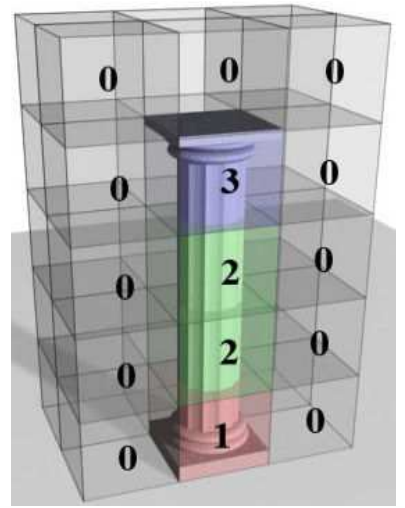
\includegraphics[width=\textwidth]{1a}
		\caption{}
		\label{fig:1a}
	\end{subfigure}
	~ %add desired spacing between images, e. g. ~, \quad, \qquad, \hfill etc. 
	%(or a blank line to force the subfigure onto a new line)
	\begin{subfigure}[b]{0.3\textwidth}
		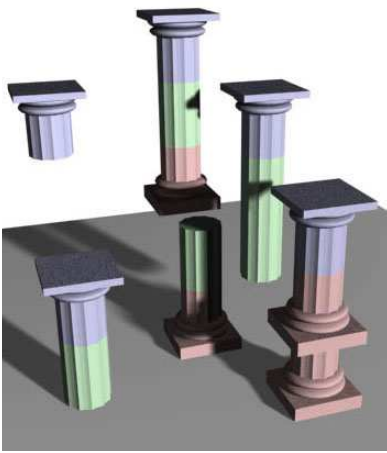
\includegraphics[width=\textwidth]{1b}
		\caption{}
		\label{fig:1b}
	\end{subfigure}
	~ %add desired spacing between images, e. g. ~, \quad, \qquad, \hfill etc. 
	%(or a blank line to force the subfigure onto a new line)
	\begin{subfigure}[b]{0.3\textwidth}
		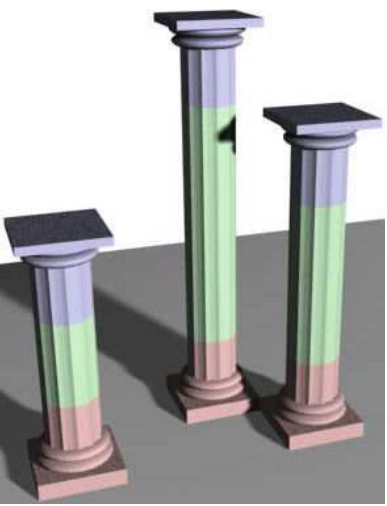
\includegraphics[width=\textwidth]{1c}
		\caption{}
		\label{fig:1c}
	\end{subfigure}
	\caption{ (a) A model composed of four model pieces, (b) An In-
		consistent Model, (c) A Consistent Model}\label{fig:animals}
\end{figure}

To check if the rules are not violated the Boolean function \textit{T} was created. This operation controls how vertices in 3D grid are labeled. If two adjacent labeled vertices are allowed to be next to one another $T(c_1,c_2) $ is equal to 1, otherwise is zero. The complete model \textit{M} is consistent only if for any two labaled vertices 
\begin{equation}
c_1,c_2 \in M, T(c_1,c_2)=1.
\end{equation}

\begin{figure}[h]
	\centering
	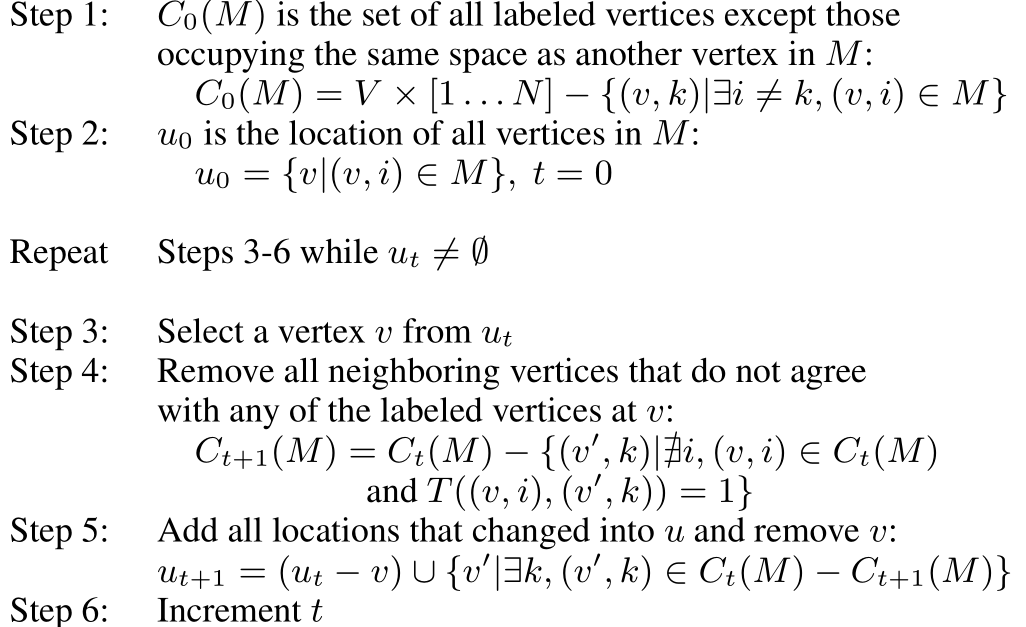
\includegraphics[width=0.85	\textwidth]{calcC}
		\caption{C(M) calculations}
	\label{CMCalc}
\end{figure}
Creating labeled vertices the conflicts will always occure. To minimize those errors the global search of conflicts was used. Algorithm will delete labaled vertices which will create conflicts from consideration. Once these labeled vertices are removed, a set of candidate labels will be create. Those candidated will be consider to add them to the model \textit{M} and this set is called $C(M)$. $C(M)$ is updated every time the model changes. Algorith to calculate $C(M)$ is provided at \figurename\ref{CMCalc}.

After the conflicts will be removed the model synthesis may start.

\begin{figure}[h]
	\centering
	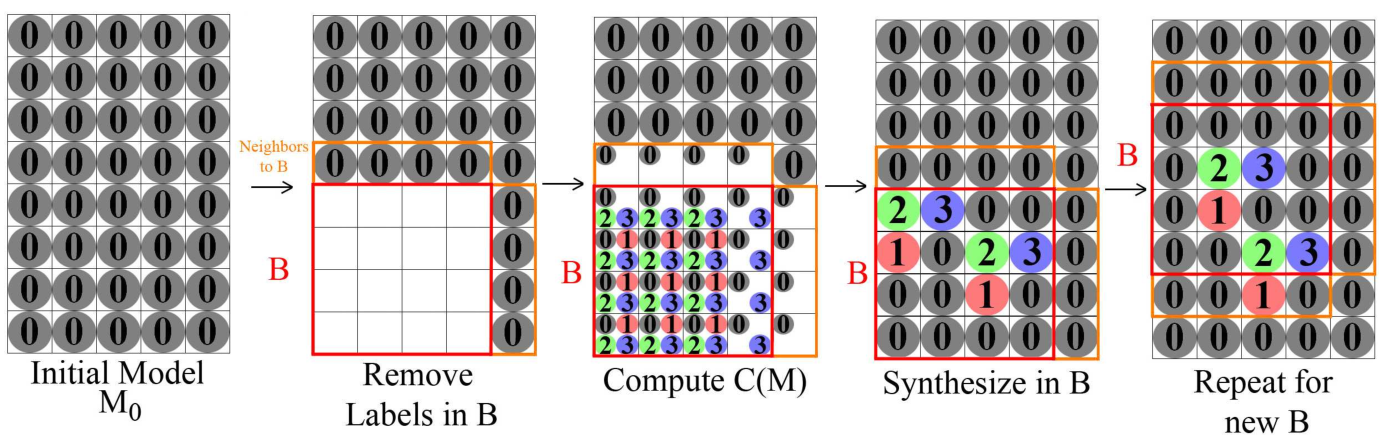
\includegraphics[width=0.9	\textwidth]{modelSynthesis}
	\caption{An example illustrating the Model Synthesis Algorithm}
	\label{ModSynth}
\end{figure}
As at \figurename\ref{ModSynth} the algorithm begin with empty space over a plane. The \textit{B} is set of vertices choosen to modify. Then the consistency is calculated at the B region, so the $C(M)$ function is used. The new model $M_0$ is created with all the old labels in B removed. For each vertex in B, a new label is selected at random from  list of candidate labels $C(M_0 )$ and assigned to the vertex. Then all steps are repeted for new region \textit{B}.

The examples of meshes created by this technique is presented at \figurename

\begin{figure}[h]
	\centering
	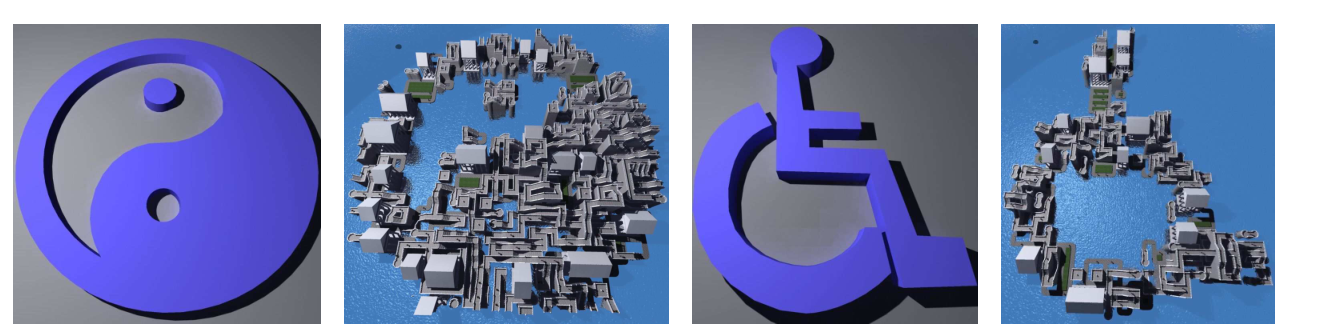
\includegraphics[width=0.9	\textwidth]{exampleMS}
	\caption{Constrained models}
	\label{exampleMS}
\end{figure}

\newpage
\section{Conclusion}

\bibliography{bib} 
\bibliographystyle{acm}
\end{document}
